\documentclass[11pt]{article}

\usepackage{amsmath, amssymb, amsfonts, amsthm}
\usepackage{hyperref}
\usepackage{mathtools}
\usepackage{centernot}
\usepackage{fancyhdr}
\usepackage{fancyvrb}
\usepackage{verbatim}
\usepackage{xcolor}
\usepackage{enumerate}
\usepackage{tikz}
\usepackage{gensymb}
\usepackage{booktabs}
\usepackage{multirow}
\usepackage{siunitx}
\usepackage[margin=0.9in,includefoot]{geometry}
\usepackage{graphicx}
\graphicspath{ {images/} }
\usepackage{longtable}
\usepackage[export]{adjustbox}
\usepackage{setspace}
\usepackage{array}
\usepackage{chngcntr}
\usepackage{pbox}
\usepackage{calc}
\usepackage{hyperref}
\usepackage{extramarks} % Required for headers and footers
\usepackage{listings,relsize}
\usepackage{csquotes}
\usepackage[shortlabels]{enumitem}
\usepackage{fancyhdr}
\usepackage{apacite}

% setup other parameters
\lstloadlanguages{R}
\pagestyle{fancy}
\fancyhf{}
\newcommand{\lil}[1]{\lstinline|#1|}
\renewcommand{\sectionmark}[1]{\markright{\thesection\ #1}}
\fancyhead[RO]{\thepage}
\pagenumbering{roman}
\counterwithin{figure}{section}
\counterwithin{table}{section}

% setup hyperlink format
\hypersetup{
  colorlinks,
  linkcolor=wine-stain,
  linktoc=all
}

% setup lstlisting format
\definecolor{wine-stain}{rgb}{0.5,0,0}
\lstdefinestyle{base}{
  language=Matlab,
  emptylines=1,
  breaklines=true,
  basicstyle=\ttfamily\color{black},
  moredelim=**[is][\color{blue}]{@}{@}
}



\begin{document}

% title page
\begin{titlepage}
   \begin{center}
   \line(1,0){450}\\
   [0.25in]
   \huge{\bfseries Statistics Learning on Rating Prediction}\\
   [2mm]
   \line(1,0){450}\\
   [0.5cm]
   \textsc{\begin{large}
   Department of Statistics and Actuarial Science\\
   University of Waterloo\\
   SPRING 2019 STAT 444
   \end{large}}\\
   \textsc{\begin{normalsize}
   \end{normalsize}}\\
   \begin{normalsize}
		\textbf{Junqi Liao} $\cdot$ \texttt{20650701} $\cdot$ \texttt{j29liao@edu.uwaterloo.ca}\\
		[2cm]
   \end{normalsize}

% abstract
\begin{abstract}
\noindent\large\onehalfspacing
In this article, we decide to carry out the prediction on the European soccer player rating. The data is extracted from the database sqlite downloaded on Kaggle. The main goal is to use various statistics learning techniques we learn in class (GAM, Smoothing Spline, Regression Tree etc.), predict players' \verb overall_rating \ based on the model we build and see which method we use has the best performance from (e.g. MSE, MSPE etc). Before implementing the algorithms, we will go through each mathematical terminology for better understanding behind its corresponding algorithm. In particular, we will discuss further improvement after we evaluate the model performance.
\end{abstract}

\end{center}
\end{titlepage}

% table of content
\tableofcontents
\thispagestyle{empty}
\cleardoublepage


% main paragraphs start here
\newpage
\setcounter{page}{1}
\pagenumbering{arabic}


% set line spacing to be 1.5
% \onehalfspacing
\singlespace

% introduction
\section{Introduction}

\subsection{Data}
The European soccer rating prediction problem on is based on a past Kaggle competition\\ (\href{https://www.kaggle.com/hugomathien/soccer}{https://www.kaggle.com/hugomathien/soccer}). This data is extracted from the European Soccer Database with 25k+ matches, 10k+ players and teams attributes for European professional football. Regarding the database, it contains everything from V1 + some fixes (missing games, full team names) and a new table with team attribute. \\

\noindent We preprocess the dataset from the file \verb database.sqlite \ extracted in the data directory. Basically, we join two tables \verb player \ and \verb player_stats \ into \verb rating_potential \ and produce the output of \verb rating_potential.csv \ file. Noted that the variable \verb gk_reflexes \ has a partial samples in the range of 65 to 85. In order to reduce the variability and maintain the normality, we basically transform that partial samples into the range of 0 to 20. The response variable \verb overall_rating \ will not be affected too much because it represents the overall average of each explanatory variable and the average will not change a lot by law of large number. We decide to use this csv file as our main data source for this project. Noticed that we will also use the variable \verb overall_rating as our target, other attributes as our explanatory variables.

\subsection{Problem}

\noindent In this project, we want to apply six modern statistics learning techniques in this article, which are multiple linear regression, LASSO Regression and ridge regression based on the assumption that the model is linear and smooth using general additive model (GAM), gradient boosting (tree-based) and regression tree based on the assumption that the model is non-parametric respectively. Here, we list the assumption and techniques below:
\begin{itemize}
\item Linear model:
\subitem- Multiple linear regression
\subitem- LASSO regression
\subitem- Ridge regression
\item Non-parametric model:
\subitem- General additive model (GAM)
\subitem- Gradient Boosting (Tree-based)
\subitem- Regression tree
\end{itemize}

\section{Exploratory Data Analysis}

\subsection{Dimension of the Dataframe}

We observe that the dimension of the dataframe \verb rating_potential \ is $10390 \times 33$. But we generally consider the subdataframe from the second column to the last column since the second column corresponds to the response variable \verb overall_rating \ and the subdataframe from the third column to the last column corresponds to input dataframe.

\subsection{Relationship between Exploratory and Response}

We first read in the table \verb rating_potential \ and display the correlation plot for each explanatory variable and corresponding response \verb overall_rating. This will give us some observation on the dataset and perspective on how to build the model, but this correlation only assumes the model is linear. We also want to observe any relationship between the explanatory variable and response variable if the model is non-linear. So we want to build both linear and non-linear model with different assumptions.\\

\begin{figure}[h]
\begin{center}
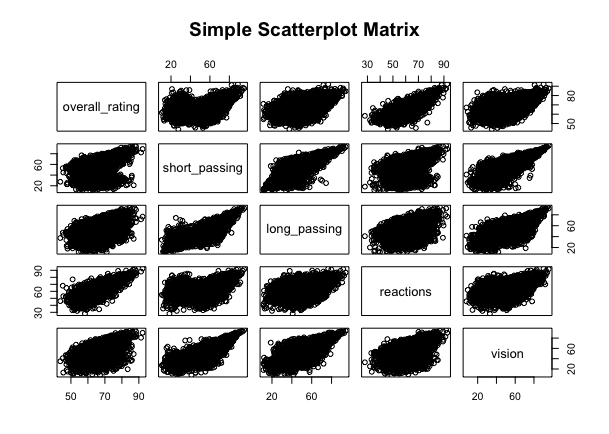
\includegraphics[height=5.7cm]{scatterplot1} \quad 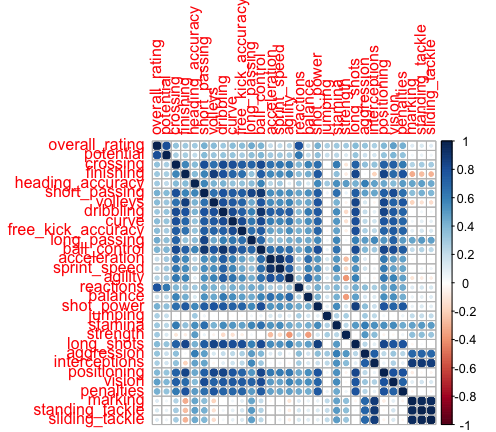
\includegraphics[height=5.7cm]{corrplot1} \quad
\caption{Scatter plot matrix and correlation plot}
\end{center}
\end{figure}

\noindent From the above scatter plot matrix and correlation plot, we notice that \verb short_passing, \verb long_passing, \\ \verb reactions  and \verb vision  have strong correlation with \verb overall_rating . This indicates that those explanatory variables mentioned above might have a great impact on the response variable \verb overall_rating \ if the model is linear in parameters.
\section{Linear Model}

In this section, we will implement the algorithms based on the assumption that the model is linear in parameters and each variable is identically independent distributed (i.i.d). Before we dig into the regression model, we did some Research and summarized each model we are going to use.

\begin{enumerate}[(1)]
\setlength\itemsep{0cm}
\item \textbf{Multiple Linear Regression} Multiple linear regression is the most common form of linear regression analysis.  As a predictive analysis, the multiple linear regression is used to explain the relationship between one continuous dependent variable and two or more independent variables.  The independent variables can be continuous or categorical (dummy coded as appropriate).

\item \textbf{LASSO Regression} Lasso regression performs L1 regularization, which adds a penalty equal to the absolute value of the magnitude of coefficients. This type of regularization can result in sparse models with few coefficients; Some coefficients can become zero and eliminated from the model. Larger penalties result in coefficient values closer to zero, which is the ideal for producing simpler models.

\item \textbf{Ridge Regression} Ridge regression is a way to create a parsimonious model when the number of predictor variables in a set exceeds the number of observations, or when a data set has multicollinearity (correlations between predictor variables). Ridge regression uses a type of shrinkage estimator called a ridge estimator. Shrinkage estimators theoretically produce new estimators that are shrunk closer to the “true” population parameters. The ridge estimator is especially good at improving the least-squares estimate when multicollinearity is present.



\end{enumerate}

\subsection{LASSO Regression}

\subsubsection{Definition}

Unlike best subset, forward stepwise, and backward stepwise selection, the main feature for LASSO is generally penalizing on the coefficient of the L1 norm. More specifically, we want to minimize the quantity:
\begin{equation*}
\min \quad \sum_{i=1}^n \bigg(y_i - \beta_0 - \sum_{j=1}^p \beta_j x_{ij}\bigg)^2 + \lambda \cdot \sum_{j=1}^p |\beta_j|
\end{equation*}

\subsubsection{Analysis}

We want to compare both of the following cases when we use LASSO:
\begin{itemize}
\item[1.] The dataset for explanatory variables is not scaled.
\item[2.] The dataset for explanatory variables is scaled.
\end{itemize}
We generally use \verb glmnet \ package to do cross validation on the training dataset. During this process, we split the dataset into 80/20, then we estimate the optimal lambda with \verb lambda.min \ and \verb lambda.1se. We then plot the optimal lambda for the first case and the second case.\\
\begin{figure}[h]
\centering
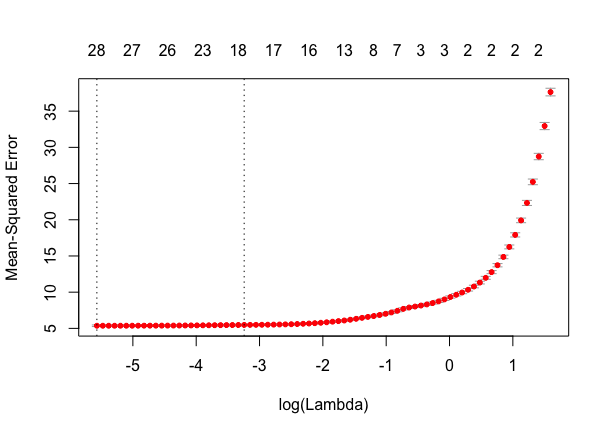
\includegraphics[height=4cm]{lassoCoefficient}\quad
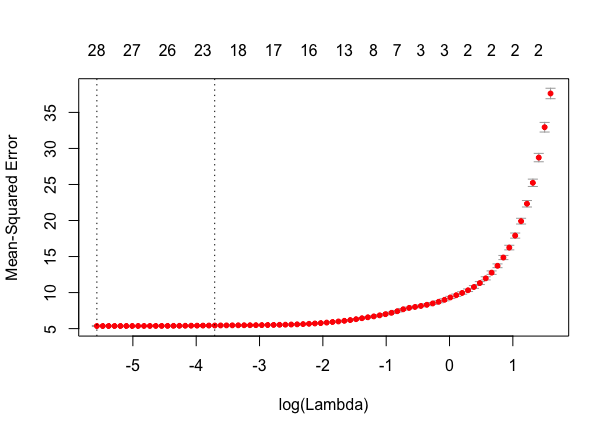
\includegraphics[height=4cm]{lassoCoefficientScaled}\caption{Optimal lambda for xtrain without scaling and with scaling}
\end{figure}

\noindent From the following figure, we observe that the optimal lambda $\lambda_{1se}$ for the first the case is relatively larger than the $\lambda_{1se}$ for the second case. The optimal lambda $\lambda_{min}$ for both cases are the same. Next, we make a table of MSE and MSPE in order to compare the performance of the models for both cases:
\begin{table}[h]
    \label{default_model}
    \centering
    \begin{tabular}{l c c}
        \hline
        \textbf{Error Type} & \textbf{Without Scaling} & \textbf{With Scaling} \\ \hline
        Mean Square Error & 5.4047726 & 5.432484 \\
        Mean Square Prediction Error  & 5.464275 & 5.506167 \\
        \hline
    \end{tabular}
    \caption{MSE and MSPE with respect to scaling and without scaling}
\end{table}
We observe that MSE for both cases are smaller than MSPE. MSE and MSPE with scaling are relatively larger than MSE and MSPE without scaling. This indicates that sometimes scaling the explanatory dataset might not be a good choice. MSE and MSPE for both cases are relatively high. So the model might be underfitting. Let's see if the MSE and MSPE would be smaller if we construct non-parametric model to predict it.


\section{Non-parametric Model}

In this section, we will implement the algorithms based on the assumption that the model is non-parametric in parameters. Before we dig into the regression model, we did some Research and summarized each model we are going to use.

\begin{enumerate}[(1)]
\setlength\itemsep{0cm}

\item \textbf{Generalized Additive Model} is to maximize the quality of prediction of a dependent variable $Y$ from various distributions, by estimating unspecific (non-parametric) functions of the predictor variables which are connected to the dependent variable via a link function.

\item \textbf{Gradient Boosting (Tree-based)} is a boosting algorithm that fits single decision tree at each iteration. Instead of averaging over all the trees, GB tries to find the best linear combination of fitted trees to explain the training data. As a result of this optimization, the GB model trains much slower but might yields better results. However it is also known to possibly overfit the training data.

\item \textbf{Regression Tree} trains very fast and works good with categorical variables. However since only one tree is fit and if the tree goes too deep, it might overfit the training data.



\end{enumerate}

\subsection{Gradient Boosting (Tree-based)}

\subsubsection{Definition}

Gradient boosting is a machine learning technique for regression and classification problems, which produces a prediction model in the form of an ensemble of weak prediction models, typically decision trees. It builds the model in a stage-wise fashion like other boosting methods do, and it generalizes them by allowing optimization of an arbitrary differentiable loss function. The general procedure is using a training set $\{(x_1,y_1),(x_2,y_2),\cdots(x_n,y_n)\}$ of known values of $x$ and corresponding values of $y$, the goal is to find an approximation $\hat F(x)$ to a function $F(x)$ that minimizes the expected value of some specified loss function $L(y, F(x))$:
\begin{equation}
\hat F = \text{argmin} \mathbb{E}_{xy}[L(y,F(x))]
\end{equation}

\subsubsection{Analysis}

\noindent For gradient Boosting, we do 75/25 splitting of training set and test set. We will generally use two tunning method to choose parameters. The first method is to use \verb caret \ package. This requires a few minutes to tune the parameters. \\
\begin{table}[h]
    \label{default_model}
    \centering
    \begin{tabular}{l c c}
        \hline
        \textbf{Parameters} & \textbf{Value} \\ \hline
        nrounds & 150 \\
        max\_depth & 3 \\
        eta & 1.0\\
        gamma & 0\\
        colsample\_bytree & 0.8\\
        min\_child\_weight & 1.0\\
        subsample & 1.0\\
        \hline
    \end{tabular}
    \caption{Tuning results using caret package}
\end{table}

\noindent although the number of iteration is relatively small from the perspective of number of samples and the shrinkage is quite large, the model finally gives us the square root of mean square error and mean square prediction error:\\
\begin{table}[h]
    \label{default_model}
    \centering
    \begin{tabular}{l c c}
        \hline
        \textbf{Error Type} & \textbf{Value} \\ \hline
        Mean Square Error & 0.890285 \\
        Mean Square Prediction Error & 1.834120 \\
        \hline
    \end{tabular}
    \caption{MSE and MSPE for the model using caret package to tune parameters}
\end{table}

\noindent Also, we want to track MSE and MSPE for each iteration, so the following also provides us with some thoughts:\\
\begin{figure}[h]
\centering
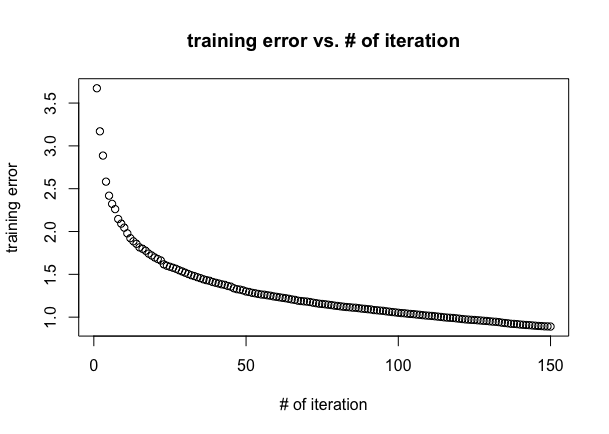
\includegraphics[height=5cm]{xgb1trainingErr}\quad
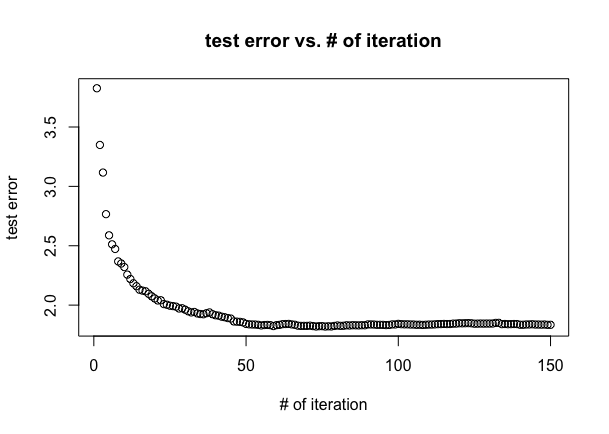
\includegraphics[height=5cm]{xgb1TestErr}\caption{Training Error and Test Error vs. \# of iteration}
\end{figure}

\noindent As we see in the figure of 4.1, when starting the iteration, the training error and test error decrease sharply. For training error, it is relatively smaller than test error and slowly decreasing after roughly the iteration of 50. For test error it is almost staying constant after the iteration of 50. This result is reasonable but it is still lack of iteration and the shrinkage is a bit large, so we also want to implement the second method using the grid search method. This method requires cross validation on the training set, setting the candidates for each tuning parameters. It will do grid searching on the whole list of tuning parameters and find the best candidates for the corresponding tuning parameters. Hence, we decide to set the following candidates of tuning parameters.\\

\begin{table}[h]
    \label{default_model}
    \centering
    \begin{tabular}{l c c}
        \hline
        \textbf{Parameters} & \textbf{Value} \\ \hline
        nrounds & [50,150,300,600,1200,2400] \\
        max\_depth & 3 \\
        eta & [0.1,0.2,0.3,0.4,0.5,0.6,0.7,0.8,0.9,1.0]\\
        gamma & 0\\
        colsample\_bytree & 0.8\\
        min\_child\_weight & 1.0\\
        subsample & 1.0\\
        \hline
    \end{tabular}
    \caption{Candidates for tuning parameters}
\end{table}

\noindent Noted that as we have more candidates for tuning the parameters, it will take some time to tune the best candidate. After we find the best candidate, \verb xgb \ also gives us trained model. This model provides the results of test RMSE for all possible candidates of parameters since we set the metric as RMSE. We want to how test RMSE behaves. Therefore, the plots of MSPE vs. \# of iteration and MSPE vs. shrinkage are provided below.\\
\begin{figure}[h]
\centering
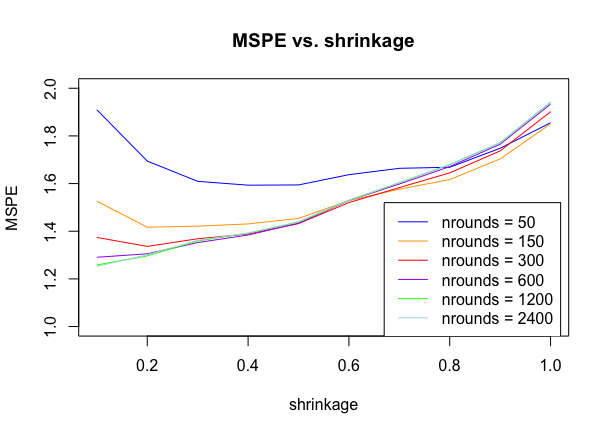
\includegraphics[height=5cm]{mspeShrinkage}\quad
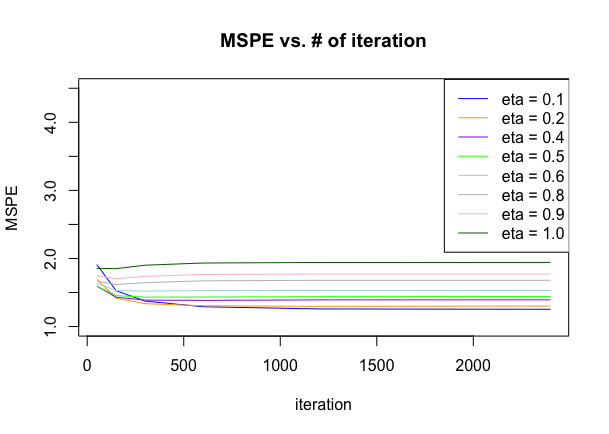
\includegraphics[height=5cm]{mspeIteration}\caption{MSPE vs. \# of iteration and MSPE vs. shrinkage}
\end{figure}

\noindent From the first figure of 4.2, if we fix a small shrinkage, when the iteration is small, the MSPE will  be larger than others, but fixing a larger shrinkage will make no difference among using each iteration as they are relatively large. From the second figure, if the shrinkage is smaller, the MSPE will decrease at the beginning of the iteration and almost will not decrease after the iteration of 500. Interestingly, MSPE for the shrinkage of 1 even increases a bit and stay almost constant after the iteration of 300. This might indicate that the model is likely to be overfitting. So it seems that smaller shrinkage, larger number of iteration gives us better model performance, but this might take some more time to train the model as the number of iteration is larger. Using the best tuning parameters we find, we have the following training error and test error for the model.\\
\begin{table}[h]
    \label{default_model}
    \centering
    \begin{tabular}{l c c}
        \hline
        \textbf{Error Type} & \textbf{Value} \\ \hline
        Mean Square Error & 0.4383072 \\
        Mean Square Prediction Error & 1.318292 \\
        \hline
    \end{tabular}
    \caption{MSE and MSPE for the model using grid search tuning}
\end{table}

\noindent From the above result, the second method gives us better performance on finding the best tuning parameter than the performance on the first one. How about their variable importance and model complexity? We plot the variable importance as follows.\\
\begin{figure}[h]
\centering
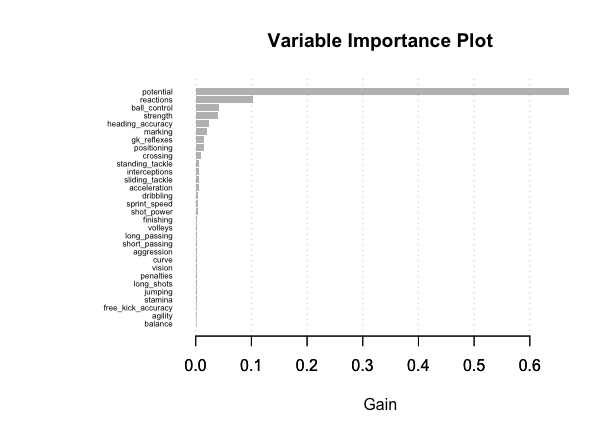
\includegraphics[height=5.5cm]{varImpXgb}\quad
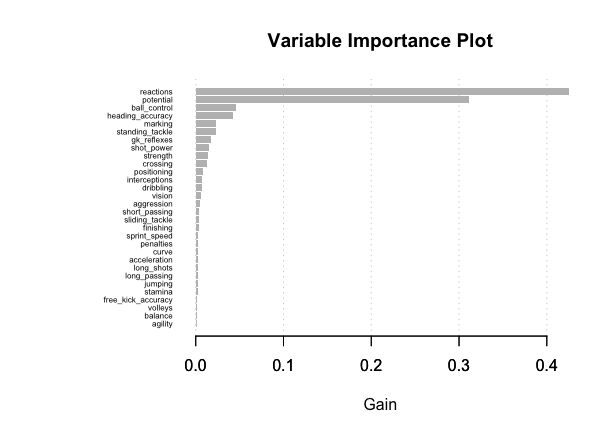
\includegraphics[height=5.5cm]{varImpXgb2}\caption{Variable importance for the first model and the second model}
\end{figure}

\noindent From the figure 4.3, we notice that the variables \verb potential \ and \verb reactions \ are relatively important for the first model. Moreover, \verb potential \ is the most important. However, for the second model, the variable \verb reactions \ is the most important. These two variable importance make sense since in the soccer match, if a soccer has a potential and a fast reaction, their team is likely to make a better shooting. We also plot the model complexity but both models have almost the same complexity with the leaf depth 4.\\

\begin{figure}[h]
\centering
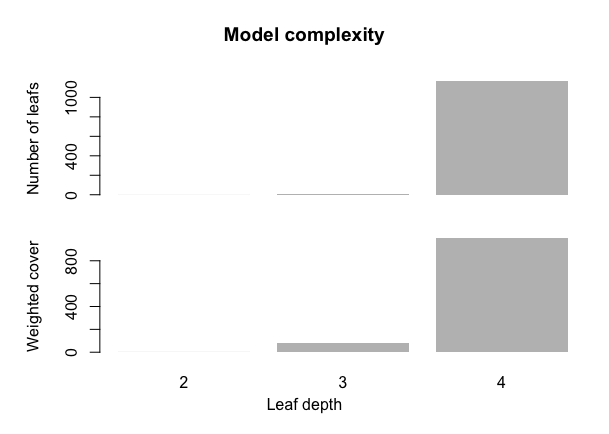
\includegraphics[height=5.5cm]{ratingboostComplexity}\quad
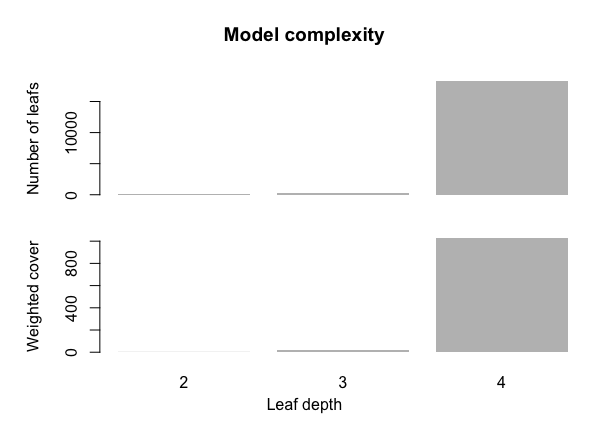
\includegraphics[height=5.5cm]{ratingboost2Complexity}\caption{Model complexity for the first model and the second model}
\end{figure}

\subsection{Generalized Additive Model}

\subsubsection{Definition}

\subsubsection{Analysis}

\noindent For Generalized Additive Model, we do 85/15 splitting of training set and test set. We will generally implement two GAMs. The first GAM is regressing on bases of functions with only one explanatory and the second GAM is regressing on bases of functions with one or two explanatories. Each two explanatory variables is represented as interaction term. First of all, we look at the first GAM. While building the first GAM, we also want to tune how many degrees of freedom for each explanatory variable term. One way to do this is to use random effects. The basic idea is to generates an i.i.d. Gaussian random effect with model matrix. For example, If \verb g \ is a factor and \verb x \ is a numeric, then \verb s(x,g,bs='re')  produces an i.i.d. normal random slope relating the response to \verb x \ for each level of \verb g. \\

\noindent For the second GAM, first we want to explore the interaction terms, but how do we do that? We generally use the \verb earth \ package to build a multiple adaptive regression spline and see which two variables highly interact with each other. From the R output of multiple hingh functions and their corresponding coefficients, we know that the interaction term could be \verb potential \ and \verb gk_reflexes , \verb dribbling \ and  \verb strength , \verb dribbling \ and \verb marking , \verb ball_control \ and \verb gk_reflexes , \verb ball_control \ and \verb gk_reflexes. After we find their interaction terms, we use the interaction function \verb ti(). From the following MSE and MSPE, we generally know that the second model performs better.\\
\begin{table}[h]
    \label{default_model}
    \centering
    \begin{tabular}{l c c c}
        \hline
        \textbf{Model} & \textbf{MSE} & \textbf{MSPE}\\ \hline
        No interaction & 1.640802 & 1.797277 \\
        With interaction & 1.320567 & 1.467482 \\
        \hline
    \end{tabular}
    \caption{MSE and MSPE for the models with interaction and without interaction}
\end{table}

\noindent checking their anova tables, we can see which smooth term has a significant non-linear effect on the response by looking at the p-value. The following are the smooth terms that are not significiant with respect to the non-linear effect.\\
\begin{table}[h]
    \label{default_model}
    \centering
    \begin{tabular}{l c c}
        \hline
        \textbf{Smooth Terms} & \textbf{p-value}\\ \hline
        s(volleys) & 0.042526 \\
        s(free\_kick\_accuracy) & 0.141044 \\
        s(agility) & 0.029730\\
        s(balance) & 0.843734\\
        s(penalties) & 0.110630\\
        \hline
    \end{tabular}
    \caption{Smooth term from the anova table}
\end{table}

\noindent From above, the smooth term s(free\_kick\_accuracy), s(balance) and s(penalties) are not significant. The smooth term s(volleys) and s(agility) are statistically significant. Other smooth terms that are not mentioned are statistically highly significant since their p-value are less than $0.01$.




\newpage



% references
\def\bibindent{1em}
\begin{thebibliography}{99\kern\bibindent}
\makeatletter
\let\old@biblabel\@biblabel
\def\@biblabel#1{\old@biblabel{#1}\kern\bibindent}
\let\old@bibitem\bibitem
\def\bibitem#1{\old@bibitem{#1}\leavevmode\kern-\bibindent}
\makeatother

% example
% \textsc{A. Paula Palacios, J. Miguel Marín, Emiliano J. Quinto, and Michael P. Wiper. (2014). \href{http://arxiv.org/pdf/1411.5780.pdf}{Bayesian modeling of bacterial growth for multiple populations}. \textit{Ann. Appl. Stat.}, Volume 8, Number 3, 1516-1537.}\\
% [0.2cm]
\textsc{Statistics How To. (n.d). Ridge regression. Retrieved on July 22nd, 2019 from : \href{https://www.statisticshowto.datasciencecentral.com/ridge-regression/}{\texttt{https://www.statisticshowto.datasciencecentral.com/ridge-regression/}}.}\\[.2cm]

\textsc{Statistics How To. (n.d). What is lasso regression? Retrieved on July 21st, 2019 from : \href{https://www.statisticshowto.datasciencecentral.com/lasso-regression/}{\texttt{https://www.statisticshowto.datasciencecentral.com/lasso-regression/}}.}\\[.2cm]

\textsc{Statistics Solutions. (n.d). What is multiple linear regression? Retrieved on July 21st, 2019 from: \href{https://www.statisticssolutions.com/what-is-multiple-linear-regression/}{\texttt{https://www.statisticssolutions.com/what-is-multiple-linear-regression/}}.}\\[.2cm]

\textsc{Statsoft. (n.d). General additive model. Retrieved on Aug 8th, 2019 from: \href{http://www.statsoft.com/Textbook/Generalized-Additive-Models}{\texttt{http://www.statsoft.com/Textbook/Generalized-Additive-Models}}.}\\[.2cm]
\end{thebibliography}
\end{document}
